\documentclass{article}

\usepackage{algorithmic}
\usepackage{amsmath}
\usepackage{graphicx}
\usepackage{hyperref}
\usepackage{booktabs}

\begin{document}

\title{Neural Network Handwriting Recognition}
\author{Geoffrey Ulman\\
        Midterm Exam\\
        CSI873}
\date{October 2011}
\maketitle

\tableofcontents

\section{Network Implementation}\label{Network Parameters}

The neural network used to classify the provided handwriting data set was a feed-forward network with 64 input nodes (one for each pixel in the input images), 10 output nodes (one for each digit 0 through 9), and one hidden layer. A number of different node counts for the hidden layer were tried and compared. The input and hidden layers also contained a threshold node whose output value was always fixed at \(1.0\). Each node in the hidden and output layers was implemented as a sigmoid threshold unit. Equation \ref{sigmoid1} demonstrates the calculations performed at a single node with inputs \(x_{0}\) through \(x_{n}\) and weights \(w_{0}\) through \(w_{n}\).

\begin{equation}\label{sigmoid1}
\begin{split}
net &= \sum\limits_{i=0}^n w_{i}x_{i}\\
\sigma_{net} &= \frac{1}{1+e^{-net}}
\end{split}
\end{equation}

The stochastic backpropagation algorithm was used to train the network. Simple experiments (described below) were performed to gain intuition about what training rates and momentum parameters worked well for this data set. A learning rate of \(0.15\) and a momentum of \(0.3\) were used for the final runs. Network weights were randomly initialized between \(-0.1\) and \(0.1\) before training began.

\begin{figure}\label{expected1}
\[ \begin{Bmatrix} 0.1 & 0.1 & 0.9 & 0.1 & 0.1 & 0.1 & 0.1 & 0.1 & 0.1 & 0.1 \end{Bmatrix} \]
\caption{Expected output vector for digit: 2}
\end{figure}

Values of \(0.9\) and \(0.1\) (instead of \(0.0\) and \(1.0\)) were used for the entries in the length 10 output vector for the training examples. This greatly reduced the tendancy of the weights to take on very large values during training (because the sigmoid has horizontal asymptotes near \(0.0\) and \(1.0\). Figure \ref{expected1} demonstrates the expected output vector for a \(2\) digit.

\section{Data Set}\label{Dataset}

The neural network described above was trained to classify \(8\) by \(8\) pixel handwriting samples with \(1\) bit of information per pixel. A total of \(930\) training samples and \(410\) testing samples was provided. Figure \ref{train_all} provides a visualization of each training sample and Figure \ref{test_all} provides a visualization of each testing sample.

\begin{figure}
\centering
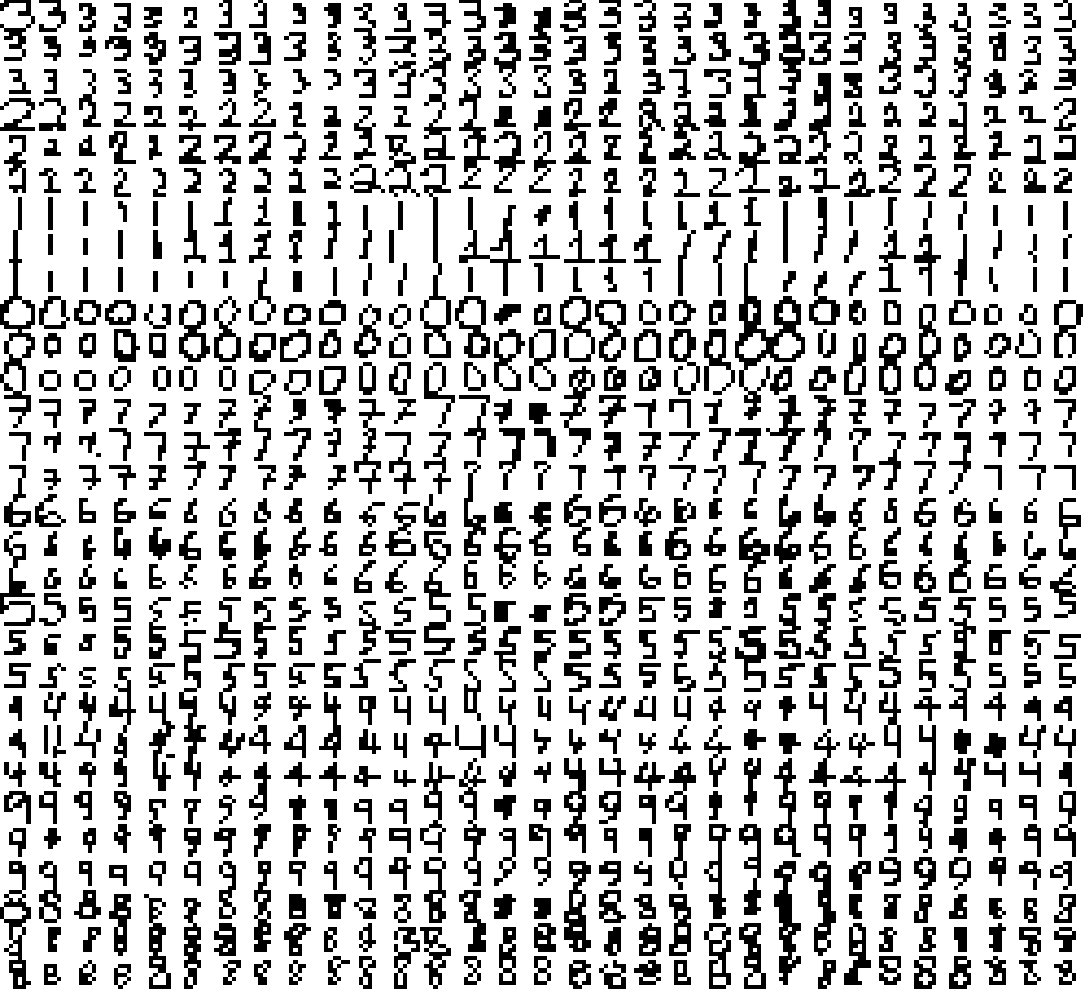
\includegraphics[width=0.85\textwidth]{data/visualization/all_training_data.png}
\caption{Handwriting samples from training data set}
\label{train_all}
\end{figure}

\begin{figure}
\centering
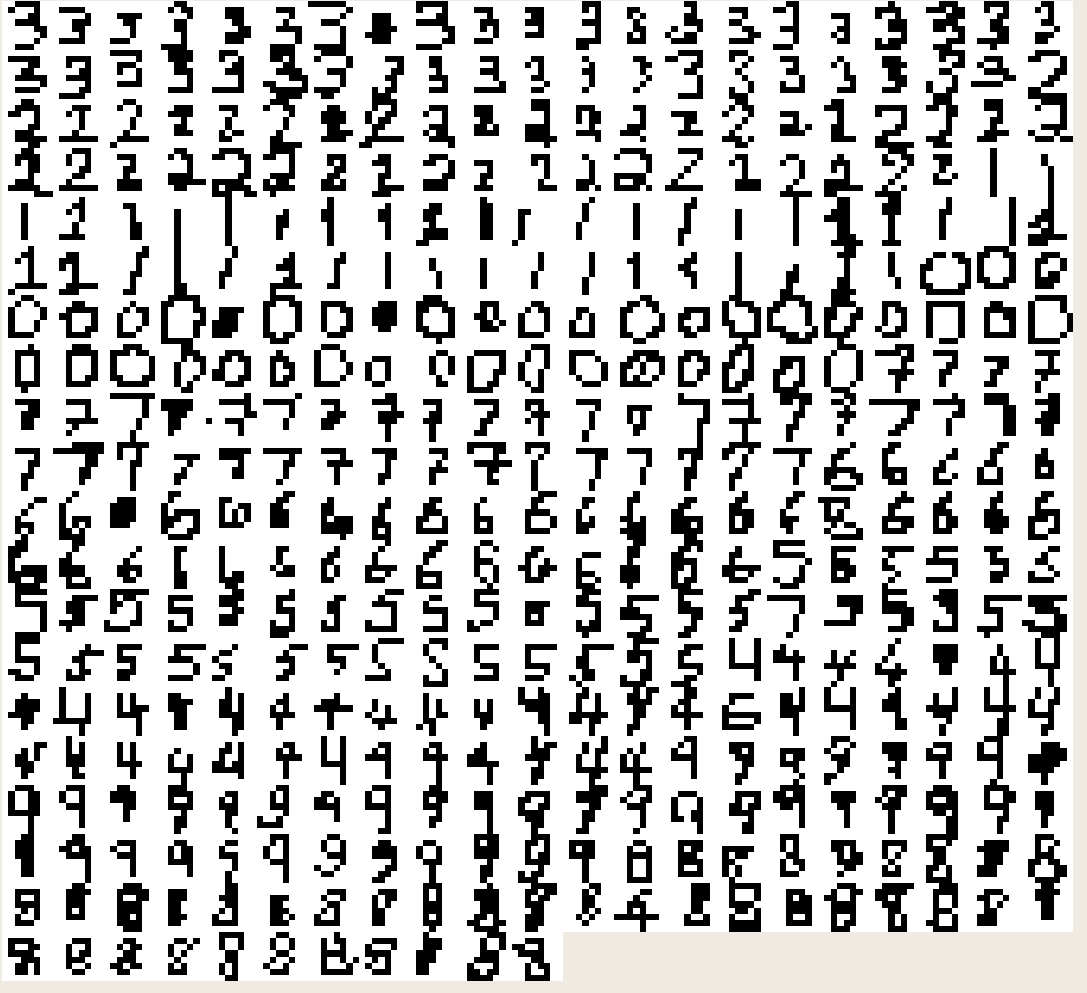
\includegraphics[width=0.85\textwidth]{data/visualization/all_testing_data.png}
\caption{Handwriting samples from test data set}
\label{test_all}
\end{figure}

\section{Software Implemenation}\label{Software Implemenation}

Java (version 1.6.0\_27) was used to implement the neural network and training algorithm. The code is available as a Subversion repository on Google Code at \url{http://code.google.com/p/csi873/}. Compiling and running the code requires the Java build tool Maven (\url{http://maven.apache.org/}). Plots were generated using the Java plotting library JFreeChart (\url{http://www.jfree.org/jfreechart/}). The Google Java general purpose Java utility library Guava (\url{http://code.google.com/p/guava-libraries/}) was also utilized for its multi-map collection data structures.

The source code is also included in the appendix and is organized with code implementing the core backpropagation algorithm and network structure up front, with less critical I/O and support code behind. Of particular interest is the Backpropagation class, which implements the stochastic backpropagation algorithm, the AbstractNet class, which handles network construction and calculation of network output, and the SigmoidNode class, which provides error, output, and weight update calculations specific to networks using a sigmoid activation function (see Equation \ref{sigmoid1}). Finnaly, the Midterm class is the main class responsible for using the components described above to load data, constructing and train a network, and output results.

Prior project work completed for CSI710 (Scientific Databases) was utilized to create the handwriting sample visualizations and confusion matrix plots. The code the visualization software is also available as a Subversion repository on Google Code at \url{http://code.google.com/p/csi701-group2/}.

\section{Results}\label{Results}

\begin{table}
\caption{Missclassification Error for 2 Hidden Node Network}
\begin{center}
\begin{tabular}{llcc}
\toprule
Data Set & Error & \multicolumn{2}{c}{95\% Confidence Interval} \\
\cmidrule(r){3-4}
& & Lower Bound & Upper Bound \\
\midrule
Testing       & 0.720 &  0.676 & 0.763  \\
Validation    & 0.760 &  0.642 & 0.878  \\
Training      & 0.702 &  0.672 & 0.732  \\
\bottomrule
\end{tabular}
\label{table2}
\end{center}
\end{table}

\begin{table}
\caption{Missclassification Error for 3 Hidden Node Network}
\begin{center}
\begin{tabular}{llcc}
\toprule
Data Set & Error & \multicolumn{2}{c}{95\% Confidence Interval} \\
\cmidrule(r){3-4}
& & Lower Bound & Upper Bound \\
\midrule
Testing       & 0.685 &  0.640 & 0.730  \\
Validation    & 0.660 &  0.529 & 0.791  \\
Training      & 0.588 &  0.555 & 0.620  \\
\bottomrule
\end{tabular}
\label{table3}
\end{center}
\end{table}

\begin{table}
\caption{Missclassification Error for 4 Hidden Node Network}
\begin{center}
\begin{tabular}{llcc}
\toprule
Data Set & Error & \multicolumn{2}{c}{95\% Confidence Interval} \\
\cmidrule(r){3-4}
& & Lower Bound & Upper Bound \\
\midrule
Testing       & 0.463 &  0.415 & 0.512  \\
Validation    & 0.440 &  0.302 & 0.578  \\
Training      & 0.345 &  0.314 & 0.377  \\
\bottomrule
\end{tabular}
\label{table4}
\end{center}
\end{table}

\begin{table}
\caption{Missclassification Error for 10 Hidden Node Network}
\begin{center}
\begin{tabular}{llcc}
\toprule
Data Set & Error & \multicolumn{2}{c}{95\% Confidence Interval} \\
\cmidrule(r){3-4}
& & Lower Bound & Upper Bound \\
\midrule
Testing       & 0.385 &  0.338 & 0.432  \\
Validation    & 0.380 &  0.245 & 0.515  \\
Training      & 0.110 &  0.090 & 0.131  \\
\bottomrule
\end{tabular}
\label{table10}
\end{center}
\end{table}

\begin{thebibliography}{9}

\bibitem{cpl}
  Brian W. Kernighan and Dennis M. Ritchie,
  \emph{The C Programming Language},
  Prentice Hall PTR, New Jersey,
  2009.

\end{thebibliography}

\end{document}
